\section{Functional Loops in Tool-Using LLMs}
\label{sec:functional-loops}

We call a feedback-visible sequence a Functional Loop when it makes no task
progress while repeating the same unresolved functional effect. This excludes
both brief inactivity and productive retries.

\textbf{Definition.} Consider a tool-use trajectory
$\tau=(s_0,a_0,o_0,\ldots,s_T)$, where $s_t$ is the online-visible interaction
state, $a_t$ is the proposed tool action, and $o_t$ is the resulting observation.
We summarize the visible task state as
\begin{equation}
q_t=(E_t,S_t,U_t),
\end{equation}
where $E_t$ is non-redundant evidence, $S_t$ is the task-relevant environment
state, and $U_t$ contains unresolved user requirements. The action effect is
\begin{equation}
e_t=(\Delta E_t,\Delta S_t,\Delta U_t,f_t),
\end{equation}
where $f_t$ records an execution or semantic failure. The mapping
$\kappa(e_t)$ canonicalizes changes to evidence, task state, unresolved
requirements, and the blocking failure.

Let $p_t=1$ when $a_t$ adds non-redundant evidence, changes state toward an
unresolved requirement, resolves a requirement, or changes a failure signature
in a way that enables a new action. For the action window
$W_{t,w}=\{t,\ldots,t+w-1\}$, define
\begin{equation}
N(t,w)=\mathbb{I}\!\left[U_t\neq\varnothing\ \land\
\sum_{j\in W_{t,w}}p_j=0\right]
\end{equation}
and
\begin{equation}
R_e(t,w)=\mathbb{I}\!\left[
\substack{\exists i<j,\ i,j\in W_{t,w}:\\
\kappa(e_i)=\kappa(e_j)\ \land\ o_i\prec a_j}
\right],
\end{equation}
where $o_i\prec a_j$ means that the earlier tool result was visible before the
later action was proposed. The strict definition is
\begin{equation}
\mathcal{L}(t,w)=N(t,w)\land R_e(t,w).
\label{eq:functional-loop}
\end{equation}
Here $N=1$ recalls a candidate, whereas $\mathcal{L}=1$ also requires a repeated
effect after feedback is visible. A loop is \emph{recoverable} only when a
Card passes grounding, abstention, and safety checks, and \emph{triggered} only
when that Card is executed. A trajectory is \emph{Functional Loop-exposed} if
it contains at least one episode. Tool strings are not part of the definition:
different tools may repeat an effect, while another call to the same tool may
produce new evidence.

\textbf{Functional Loop variation by model and benchmark.}
Figures~\ref{fig:statebench-model-fl} and~\ref{fig:cross-benchmark-fl} separate
two sources of variation. On the same failed STATE-Bench tasks, Qwen3-14B
loops more often than DeepSeek-v4-Flash, MiMo-v2.5-Pro, or DeepSeek-v4-Pro.
With DeepSeek-v4-Flash held fixed, prevalence is highest on DeepPlanning
Shopping, lower on $\tau$-Knowledge, and lowest on STATE-Bench. Functional
Loops therefore depend on both the model's tool policy and the environment.

\begin{figure}[t]
  \centering
  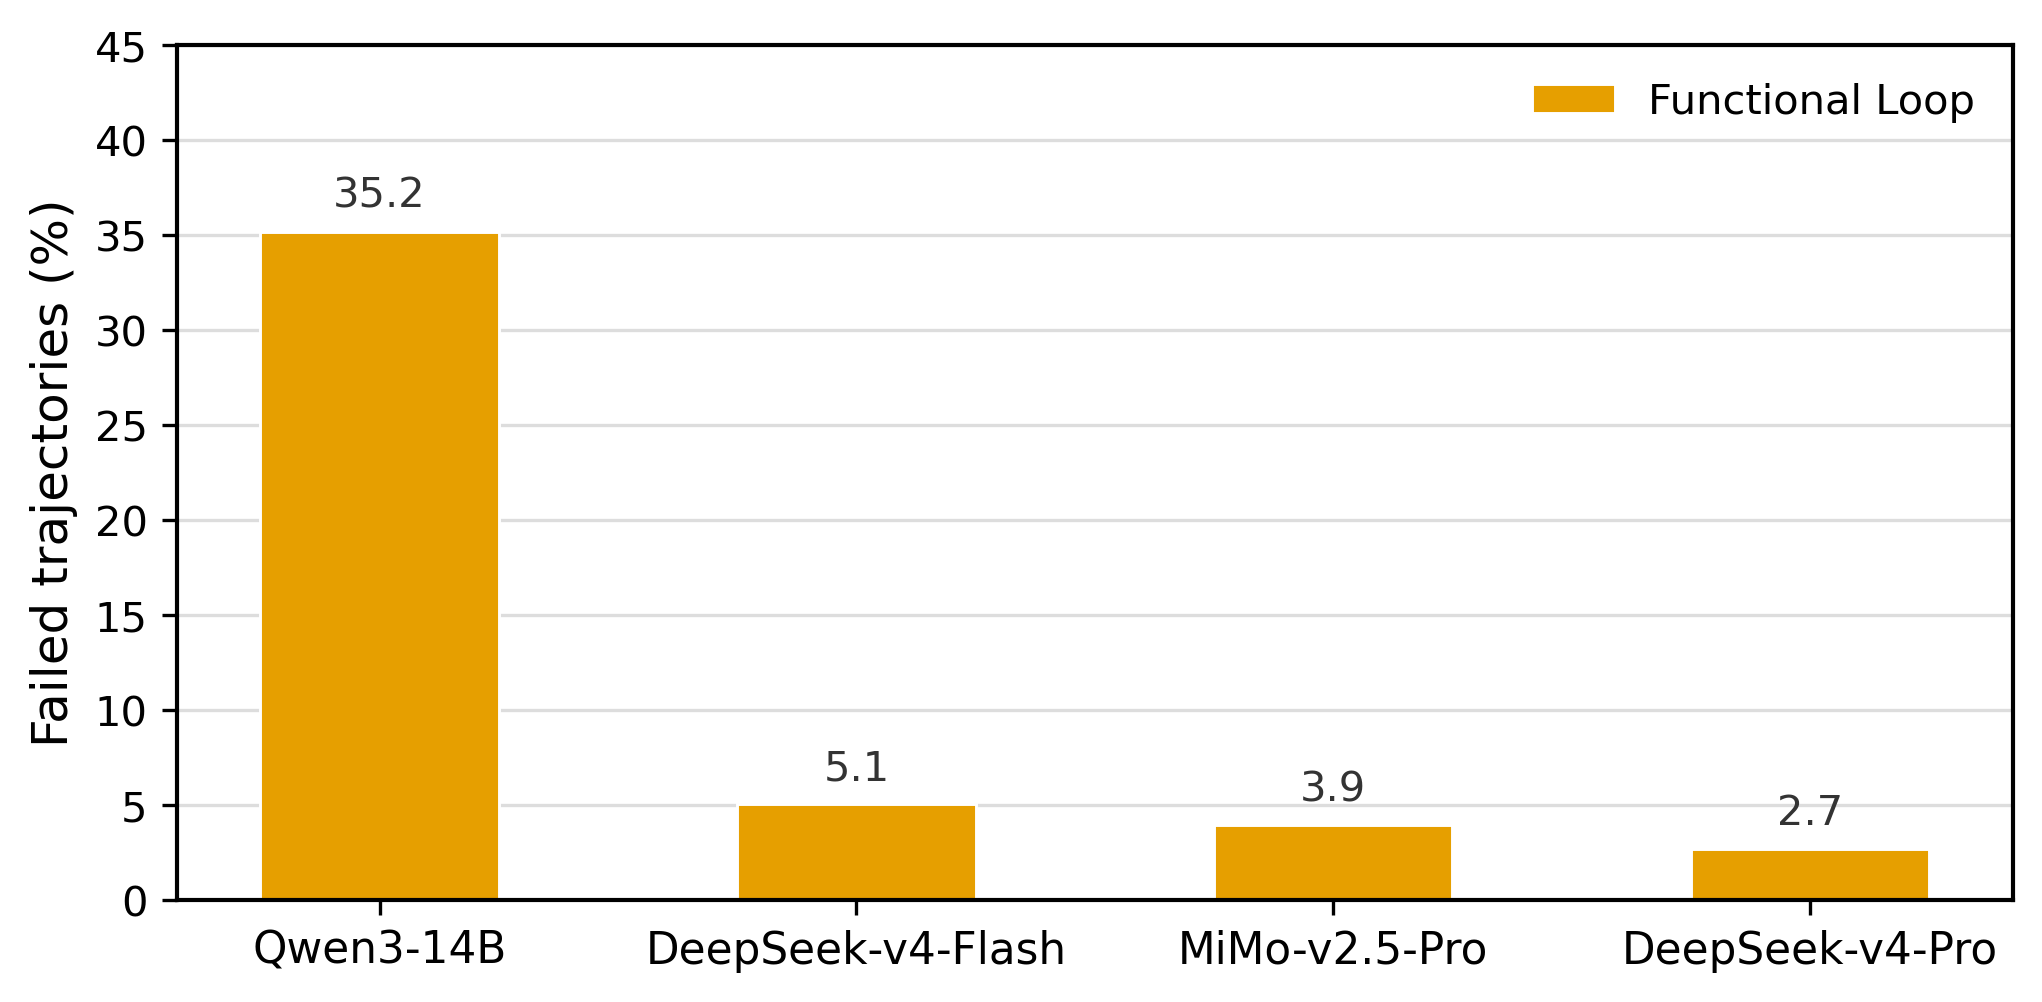
\includegraphics[width=\columnwidth]{figures/fig_statebench_fl_or_invalid_models.png}
  \caption{Functional Loop prevalence among failed STATE-Bench trajectories
  for four tool-using LLMs.}
  \label{fig:statebench-model-fl}
\end{figure}

\begin{figure}[t]
  \centering
  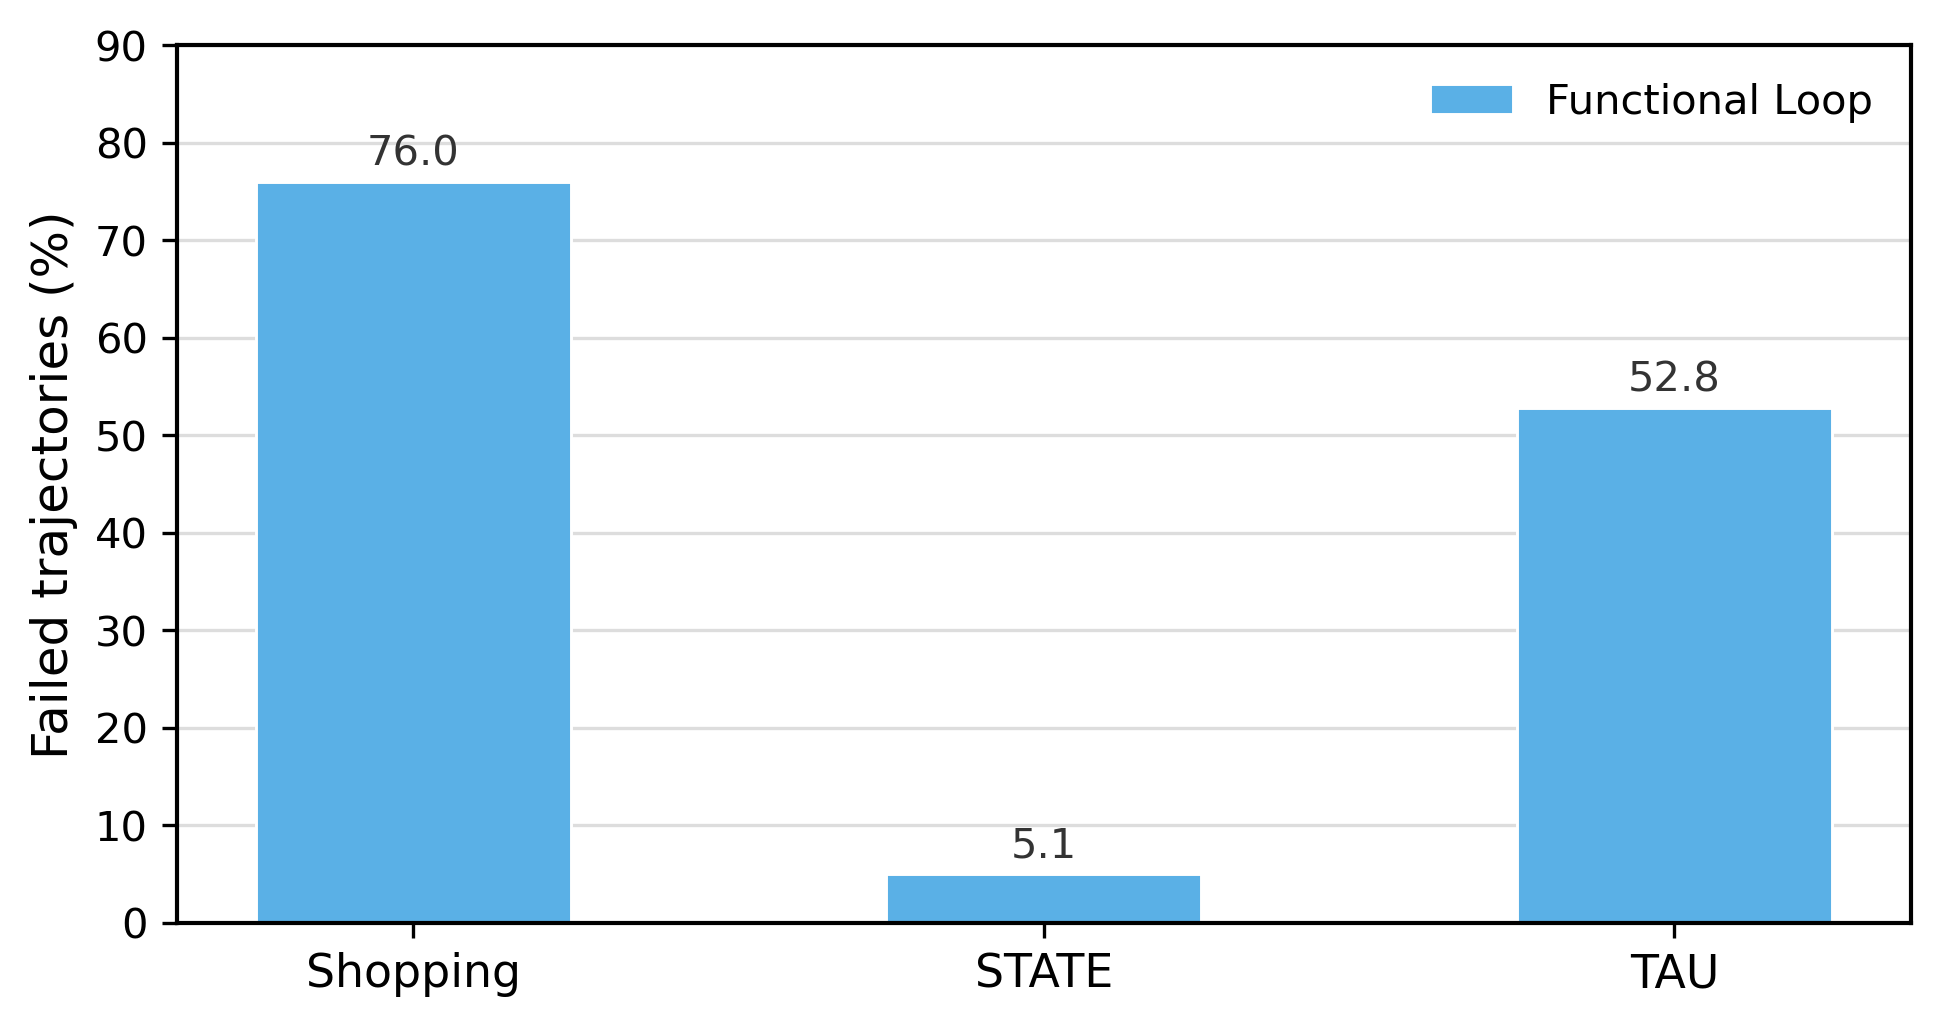
\includegraphics[width=\columnwidth]{figures/fig_cross_benchmark_fl_fixed_agent.png}
  \caption{Functional Loop prevalence among failed DeepSeek-v4-Flash
  trajectories on three benchmarks.}
  \label{fig:cross-benchmark-fl}
\end{figure}

\textbf{Functional Loops, outcomes, and cost.}
On STATE-Bench, Functional Loop-exposed trajectories have lower scores and use
more tool calls for every evaluated model
(Figure~\ref{fig:statebench-fl-consequence}). This is an observational
association: difficult tasks may both invite longer interaction and fail more
often. Even so, the pattern identifies a costly execution state worth
recovering from.

\begin{figure}[t]
  \centering
  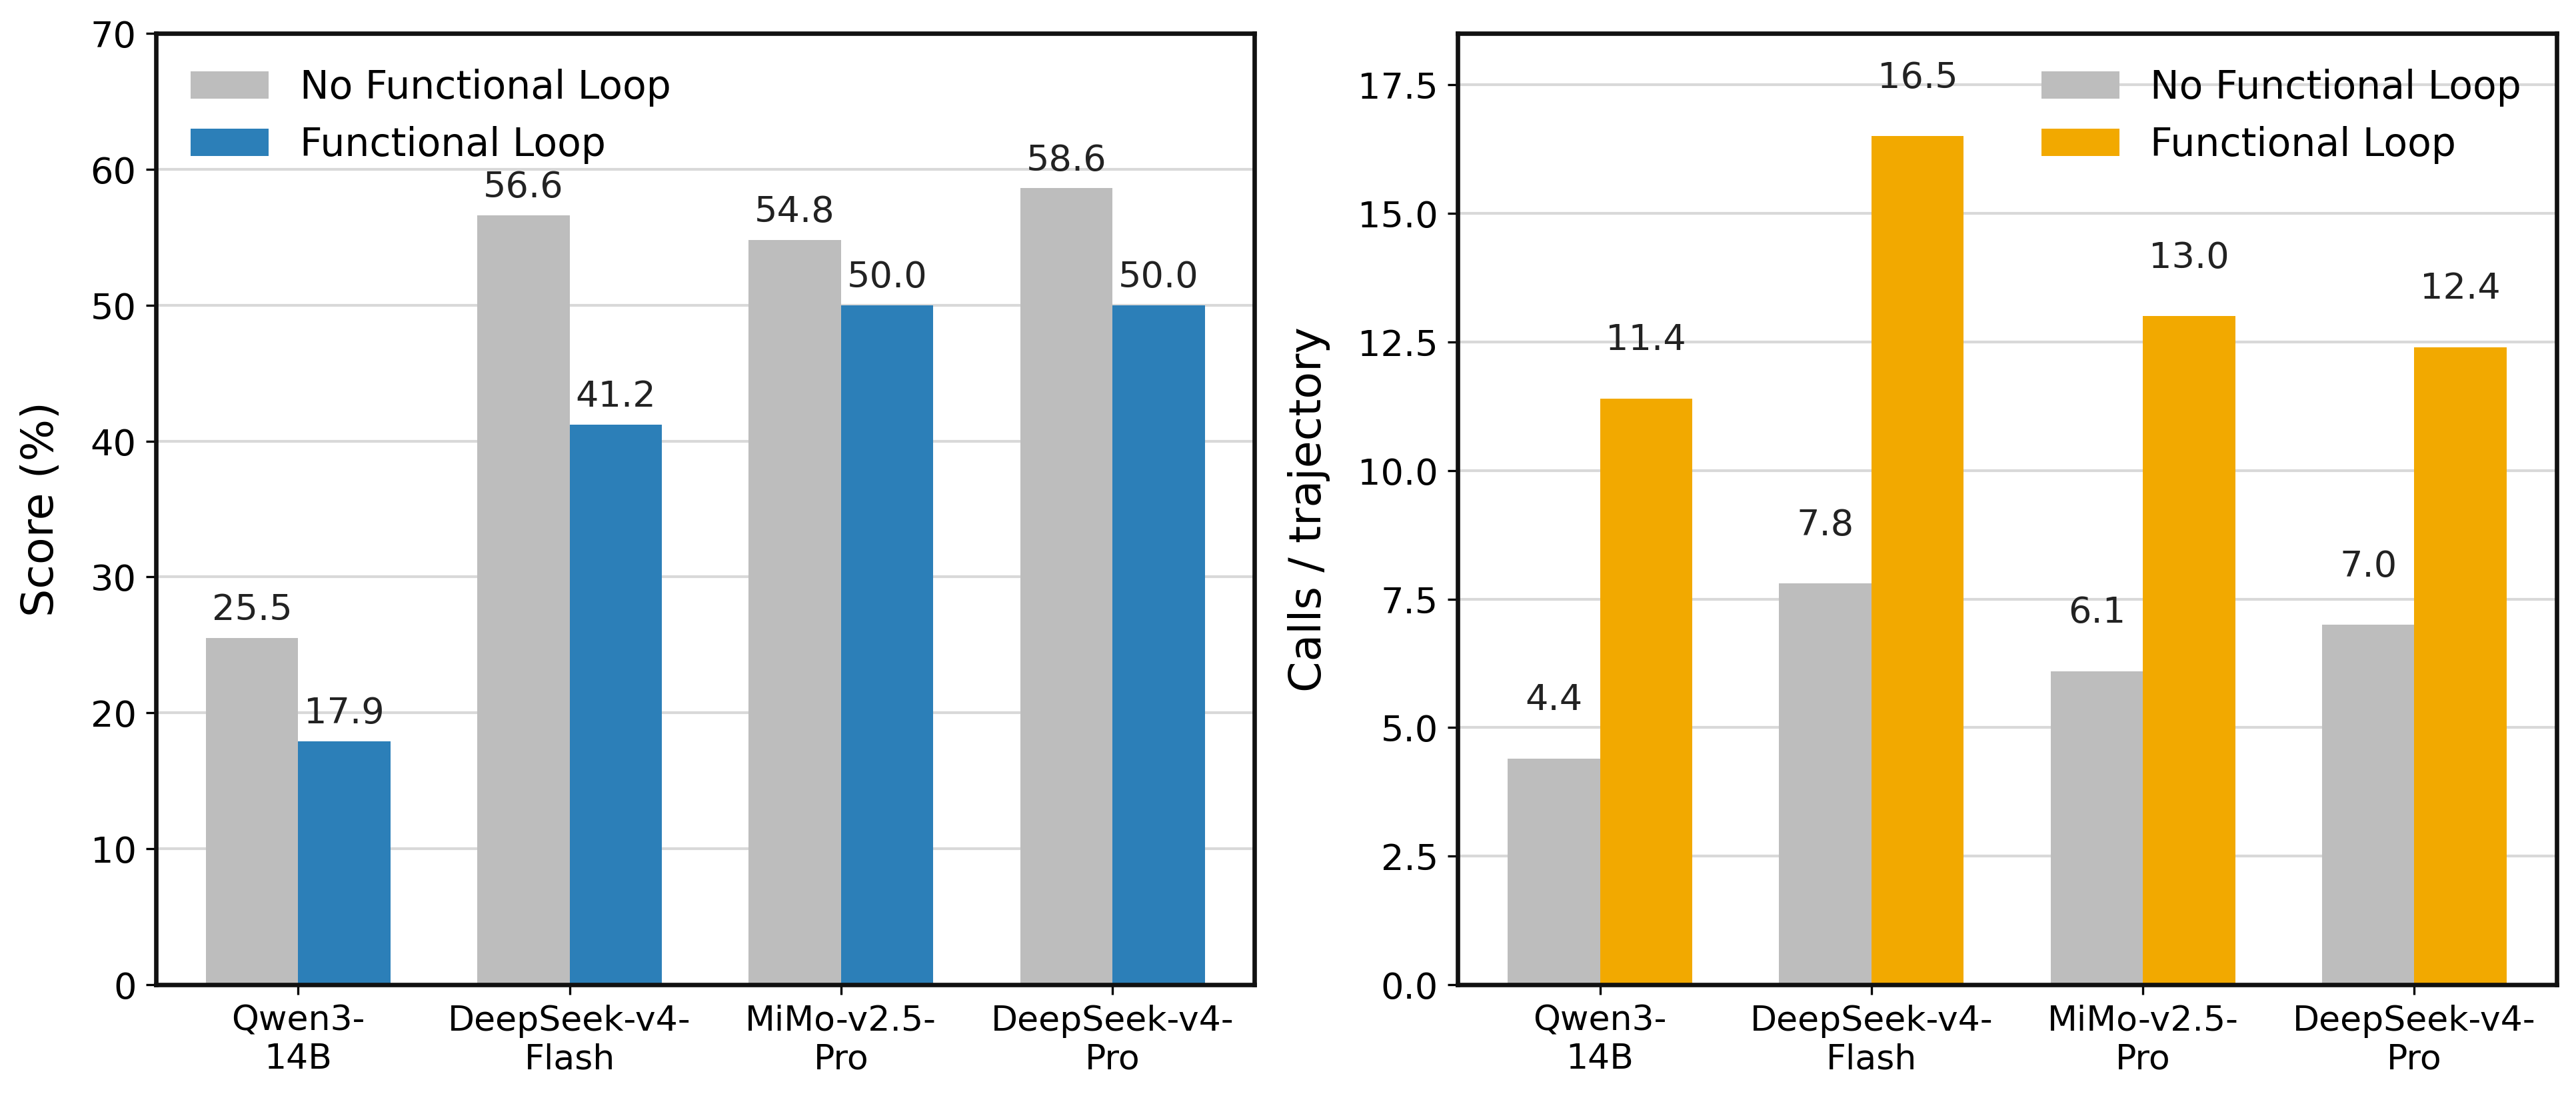
\includegraphics[width=\columnwidth]{figures/fig_fl_statebench_consequences.png}
  \caption{STATE-Bench outcomes and tool calls grouped by Functional Loop
  exposure. }
  \label{fig:statebench-fl-consequence}
\end{figure}

Consecutive reuse of the same tool gives a weaker signal
(Figure~\ref{fig:same-tool-repeat}): score differences are small and change
direction across models. Functional effects, rather than action strings,
provide the useful boundary.

\begin{figure}[t]
  \centering
  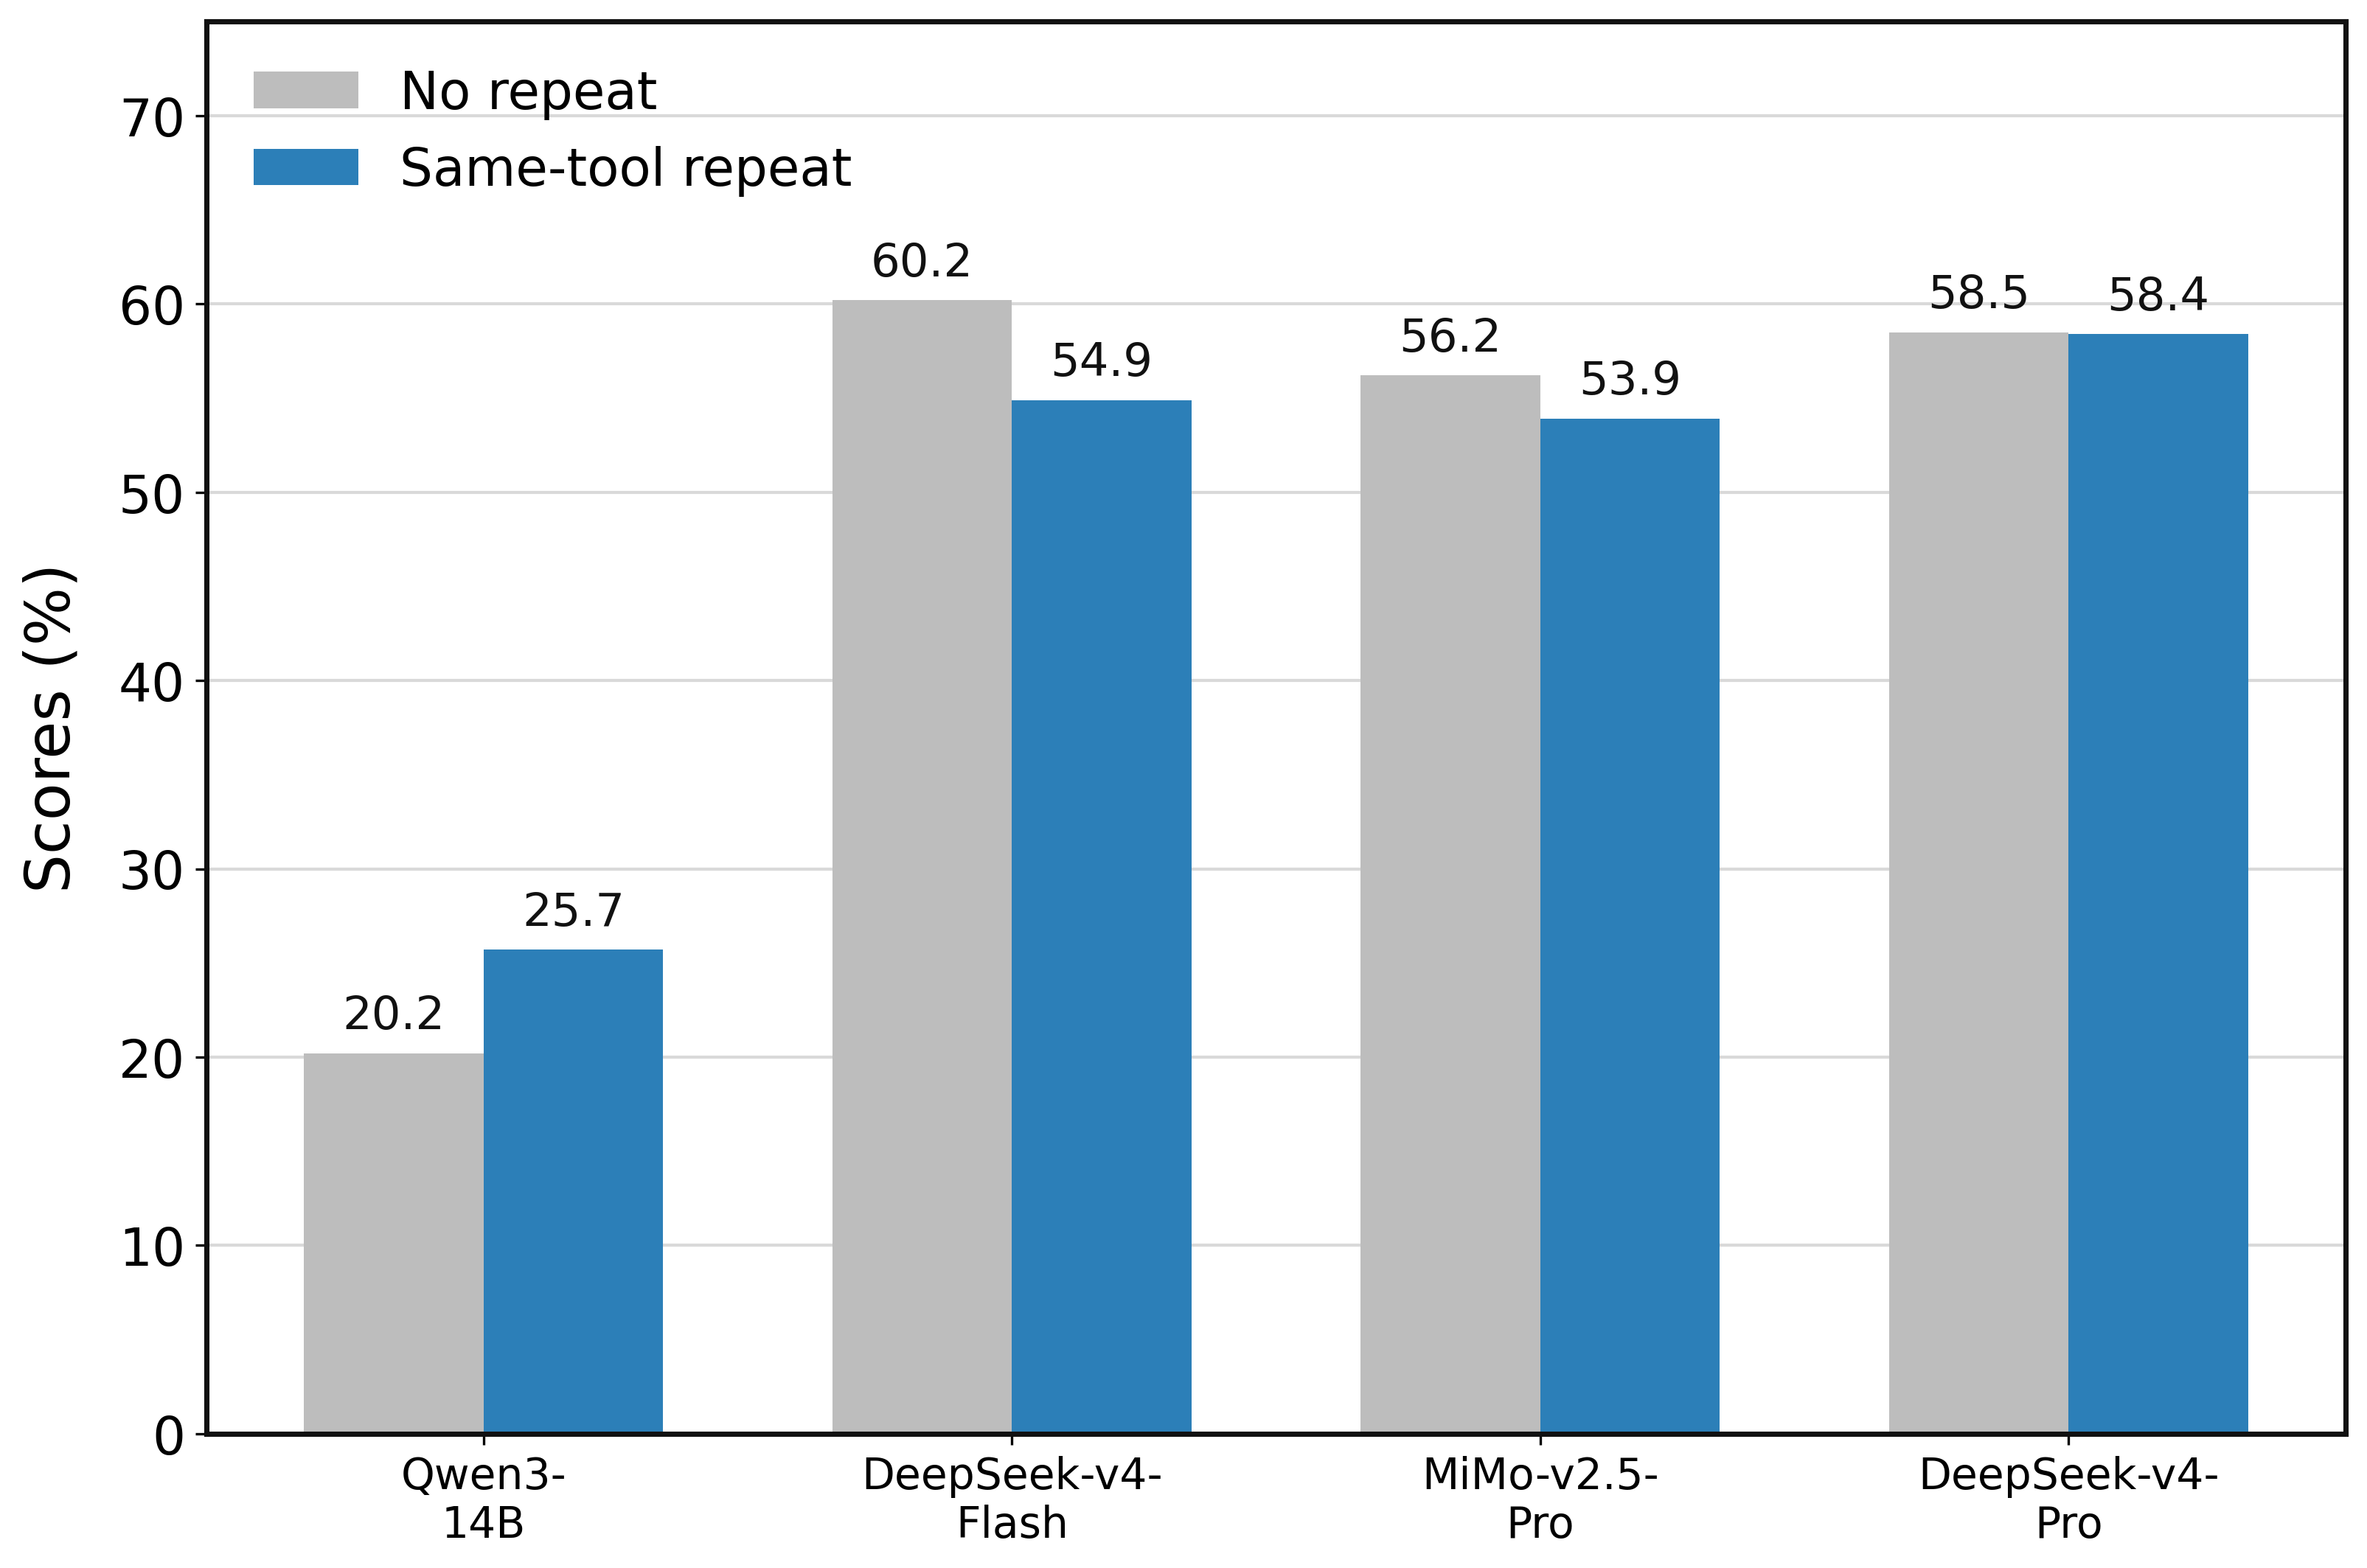
\includegraphics[width=\columnwidth]{figures/fig_statebench_same_tool_repeat.png}
  \caption{Raw STATE-Bench score grouped by consecutive calls with the same
  tool name. String-level repetition is a weak proxy for unresolved effect.}
  \label{fig:same-tool-repeat}
\end{figure}

\textbf{Case study: a cross-tool Functional Loop.}
Table~\ref{tab:cross-tool-fl-case} traces a Raw STATE-Bench Shopping
trajectory in which DeepSeek-v4-Flash searches for wireless headphones under
a hard \$100 budget. Two valid searches find nothing; the LLM then retrieves a
\$110 item and checks its details, the account, and promotions. The tools
change, but none resolves the budget constraint.

\begin{table}[t]
\centering
\scriptsize
\setlength{\tabcolsep}{2pt}
\begin{tabular}{@{}p{0.08\columnwidth}p{0.29\columnwidth}p{0.28\columnwidth}p{0.27\columnwidth}@{}}
\toprule
Step & Tool action & Feedback & Functional effect \\
\midrule
1--2 & \texttt{search\_products} ($\leq\$100$) & No matching headphones & No feasible item \\
3 & \texttt{search\_products} ($\leq\$1000$) & Finds a \$110 candidate & Budget violated \\
4 & \texttt{get\_product}\newline\texttt{\_details} & Confirms the \$110 price & Violation persists \\
5--6 & Account and promotion queries & No benefit or discount & Constraint unresolved \\
\bottomrule
\end{tabular}
\caption{A cross-tool Functional Loop from STATE-Bench Shopping. Different
calls repeat the same unresolved budget effect after feedback is visible.}
\label{tab:cross-tool-fl-case}
\end{table}

The first searches are productive because they may reveal a feasible item. The
loop begins only after the over-budget candidate is known and subsequent checks
add no repair evidence. It is a recovery signal, not an automatic stop command.

\textbf{From Functional Loop signals to recovery.}
No progress recalls a candidate; a feedback-visible repeated effect establishes
the loop; admission then asks whether a unique, grounded repair is available.
PERSIST-ACE executes one bounded Card only when these checks pass and then
returns control to the LLM. Figure~\ref{fig:escape-example} illustrates the
escape, while Figure~\ref{fig:framework} implements it as
Observe--Detect--Admit--Recover.
